\section{Cơ sở lý thuyết}

\subsection{Ảnh số}

Ảnh $f(x,y)$ được miêu tả bằng những mẫu cách đều nhau ở dạng ma trận $(N-M)$:

$$f(x,y) \begin{bmatrix}
f(0,0) & f(0,1) & \cdots & f(0,M-1) \\
f(1,0) & f(1,1) & \cdots & f(1,M-1) \\
\cdots & \cdots & \cdots & \cdots \\
f(N-1,0) & f(N-1,1) & \cdots & f(N-1,M-1) \\
\end{bmatrix} = A$$

Ma trận A được gọi là ảnh số, mỗi thành phần của A được gọi là một điểm ảnh, hay pixel.

\textbf{Lấy mẫu}: chia mặt phẳng $xy$ thành mắt lưới, tọa độ của mỗi mắt lưới là $(x,y)$, trong đó $x,y$ là số nguyên.

\textbf{Lượng tử hóa}: $f$ được gán bằng một giá trị mức xám $G$ (thực hoặc nguyên).

\textbf{Độ phân giải} cho biết mức độ chi tiết của ảnh. Độ phân giải có thể phân loại thành (1) độ phân giải không gian và (2) độ phân giải mức xám.

\begin{enumerate}
    \item Độ phân giải không gian: là chi tiết nhỏ nhất có thể nhìn thấy được trong một hình ảnh. 
    Độ phân giải không gian phụ thuộc vào số lượng điểm ảnh. 
    Yếu tố chính quyết định độ phân giải không gian là lấy mẫu.

    \item Độ phân giải mức xám: đề cập đến sự thay đổi nhỏ nhất có thể nhận thấy được trong mức xám.
    Độ phân giải mức xám phụ thuộc vào số lượng mức xám.
\end{enumerate}

\begin{figure}[H]
    \centering
    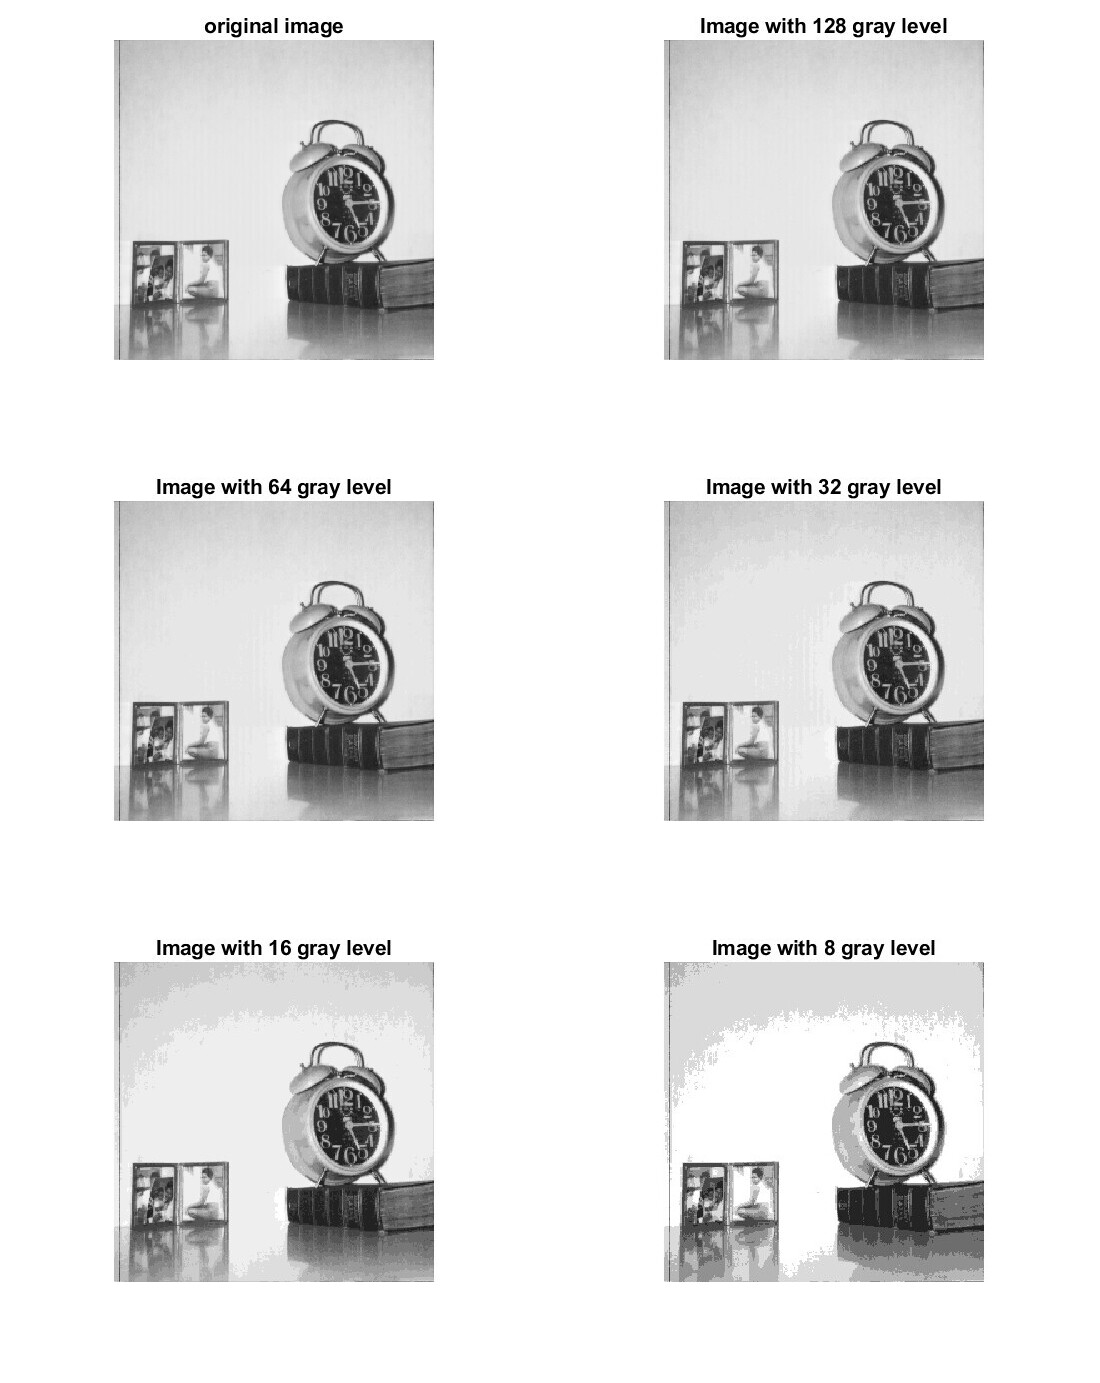
\includegraphics[width=.75\linewidth]{images/gray_scale_resolution.jpg}
    \caption{Ảnh xám với các độ phân giải mức xám khác nhau}
    \label{fig:gray_scale_resolution}
\end{figure}

\subsection{Phép toán giữa các điểm ảnh}

Các phép toán số học và logic trên hai ảnh được thực hiện trên từng điểm ảnh.
Các phép toán này chỉ thực hiện được nếu hai ảnh có cùng kích thước, nhưng nếu điều này không thỏa, ta vẫn có thể thực hiện các phép toán này trên vùng giao của hai ảnh. Nếu hai ảnh có kích thước $w_1 \times h_1$ và $w_2 \times h_2$ và giả sử gốc tọa độ của chúng giống nhau, vậy kết quả của phép toán trên hai ảnh này sẽ có kích thước $w \times h$, trong đó:

\begin{align}
    w &= \min (w_1, w_2) \\
    h &= \min (h_1, h_2)
\end{align}

\textbf{Phép cộng và trừ ảnh}

Cho hai ảnh $x_1$ và $x_2$ có vùng giao nhau có kích thước $W \times H$, $y$ là kết quả của phép toán giữa hai điểm ảnh, và các ảnh đều có độ phân giải mức xám N bit. Ta có các phép toán cộng và trừ giữa hai ảnh như sau:

\begin{align}
    y(i,j) &= \min \{ x_1(i,j) + x_2(i,j), 2^N \} \\
    y(i,j) &= \| x_1(i,j) - x_2(i,j) \|
\end{align}

Trong đó, $0 \leq i \leq H-1$ và $0 \leq j \leq W-1$.

Phép cộng ảnh có ứng dụng trong việc giảm nhiễu hình ảnh bằng cách lấy trung bình nhiều quan sát của cùng một khung hình. 
Phép trừ ảnh có ứng dụng trong việc phát hiện chuyển động, thông qua phân tích các điểm ảnh có giá trị khác không sau khi thực hiện phép trừ.

\textbf{Phép nhân và chia ảnh với một số}

Cho ảnh $x$ là ảnh thực hiện phép toán và ảnh $y$ là kết quả, có cùng kích thước và độ phân giải mức xám $N$ bit.
Phép nhân ảnh với một số $k$ được biểu diễn như sau:

\begin{equation}
    y(i,j) = k x(i,j) \quad (0 \leq i \leq H-1, 0 \leq j \leq W-1)
\end{equation}

Phép chia ảnh với một số tương tự như phép nhân, trong đó $|k| < 1$.

Phép nhân và chia các điểm ảnh với một số có thể được dùng để điều chỉnh độ sáng của một ảnh. Nhân các điểm ảnh với một số lớn hơn một sẽ làm sáng ảnh, và chia các điểm ảnh với một số lớn hơn mợt sẽ làm tối ảnh. Nhân (hoặc chia) các điểm ảnh với một số âm sẽ làm đảo màu của ảnh.

\textbf{Phép tích chập}: Tích chập rời rạc hai chiều giữa hai tín hiệu $x[n_1, n_2]$ và $h[n_1, n_2]$ là: 

$$y(n_1,n_2) = \sum_{k_1 = -\infty}^{+\infty} \sum_{k_2 = -\infty}^{+\infty} x(k_1,k_2) h(n_1-k_1, n_2-k_2)$$

Ở góc nhìn khác, phép tích chập hai chiều trong ảnh số chính là tính toán giá trị mới của điểm ảnh dưới dạng tổng có trọng số của các giá trị điểm ảnh trong một vùng lân cận nhất định xung quanh nó.

Tích chập có thể được sử dụng để thực hiện quá trình lọc tuyến tính.

\subsection{Một số loại loại nhiễu ảnh thường gặp}

\subsubsection{Nhiễu Gauss}

Nhiễu Gauss là nhiễu có hàm mật độ xác suất là phân phối Gauss. Nói cách khác, các giá trị mà nhiễu có thể nhận được phân bố theo Gauss.

Hàm mật độ xác suất $p$ của một biến ngẫu nhiên Gauss được cho bởi

$$p(z) = \frac{1}{\sqrt{2\pi} \sigma}e^{-(z-\bar{z})^2 / 2\sigma^2}$$

Trong đó $\sigma^2$ là phương sai và $\bar{z}$ là giá trị trung bình.

Các nguồn nhiễu Gauss chính trong ảnh số phát sinh trong quá trình thu thập. Cảm biến vốn có nhiễu do mức độ chiếu sáng và nhiệt độ của chính nó, đồng thời các mạch điện tử được kết nối với cảm biến cũng tạo ra phần nhiễu riêng của chúng.

\subsubsection{Nhiễu muối tiêu}

\textit{Nhiễu muối tiêu} hay còn gọi là \textit{nhiễu xung} là một dạng nhiễu đôi khi được thấy trên ảnh số. Nhiễu này có thể được gây ra bởi sự nhiễu loạn rõ rệt và đột ngột trong tín hiệu ảnh. Nhiễu này được thể hiện dưới dạng các điểm ảnh trắng và đen xuất hiện thưa thớt.

\begin{figure}[H]
    \centering
    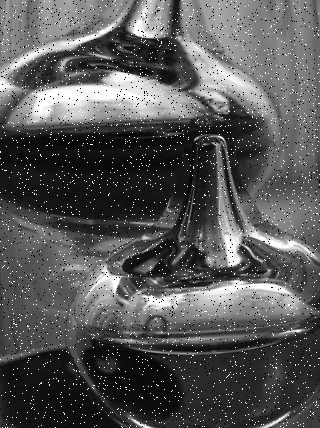
\includegraphics[width=0.5\linewidth]{images/salt_and_pepper_noise.png}
    \caption{Một ảnh với nhiễu muối tiêu}
    \label{fig:salt_and_pepper_noise}
\end{figure}

Hàm mật độ xác suất của nhiễu muối tiêu được cho bởi

$$p(z) = \left\{\begin{matrix}
P_a & z = a \\
P_b & z = b \\
0 & \text{khác} \\
\end{matrix}\right.$$

Trong đó $a = 0$ và $b = 255$ đối với ảnh mức xám 8 bit.

% \subsubsection{Nhiễu tuần hoàn}

% Một nguồn nhiễu tuần hoàn phổ biến trong ảnh là do nhiễu điện trong quá trình chụp ảnh. 
% Một ảnh bị ảnh hưởng bởi nhiễu tuần hoàn sẽ trông như một mẫu lặp lại đã được thêm lên trên ảnh gốc. 
% Trong miền tần số, loại nhiễu này có thể được coi là các xung rời rạc. 

% \begin{figure}[H]
%     \centering
%     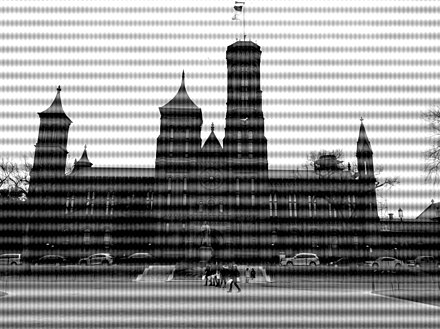
\includegraphics[width=0.75\linewidth]{images/periodic_noise.jpg}
%     \caption{Một ảnh với nhiễu tuần hoàn}
%     \label{fig:periodic_noise}
% \end{figure}

\subsection{Các loại bộ lọc}

Trong xử lý ảnh, một bộ lọc (hay còn gọi là kernel, ma trận tích chập, hay mặt nạ) là một ma trận có kích thước nhỏ so với kích thước ảnh cần được lọc, được ứng dụng trong việc làm mờ ảnh, sắc nét ảnh, phát hiện cạnh... 
Việc lọc ảnh được thực hiện bằng cách lấy tích chập giữa một bộ lọc và một ảnh. 
Một cách đơn giản, điểm ảnh ngõ ra là một hàm của các điểm ảnh ngõ vào lân cận (bao gồm cả chính nó).

Gọi $x(i,j)$ là ảnh gốc, $y(i,j)$ là ảnh sau khi lọc. Bộ lọc $h$ có kích thước $W_\text{filter} \times H_\text{filter}$. $S_{ij}$ là tập con của ngõ vào chứa các điểm lân cận xung quanh $(i,j)$:

$$S_{ij} = \begin{bmatrix}
x[i-m,j-n] & \cdots & x[i-m,j] & \cdots & x[i-m,j+n] \\
\vdots &  & \vdots &  & \vdots \\
x[i,j-n] & \cdots & x[i,j] & \cdots & x[i,j+n] \\
\vdots &  & \vdots &  & \vdots \\
x[i+m,j-n] & \cdots & x[i+m,j] & \cdots & x[i+m,j+n] \\
\end{bmatrix}, \quad m = \frac{H_\text{filter}}{2}, n = \frac{W_\text{filter}}{2}$$

Ta có biểu diễn tường minh của một số bộ lọc như sau:

Bộ lọc trung vị:

$$y(i,j) = \text{median}_{(s,t) \in S_{ij}}{\{x(s,t)\}}$$

Bộ lọc max:

$$y(i,j) = \max_{(s,t) \in S_{xy}}{\{x(s,t)\}}$$

Bộ lọc min:

$$y(i,j) = \min_{(s,t) \in S_{xy}}{\{x(s,t)\}}$$

Bộ lọc trung điểm:

$$y(i,j) = \frac{1}{2} \left ( \min_{(s,t) \in S_{xy}}[x(s,t)] + \max_{(s,t) \in S_{xy}}[x(s,t)]\right )$$